\documentclass[tikz,border=2pt,11pt]{standalone}
\usetikzlibrary{arrows.meta}
\usetikzlibrary{calc}
\usetikzlibrary{positioning}
\usetikzlibrary{fit}
\usepackage{amsmath}
\usepackage{amssymb}
\usepackage{xcolor}
\usepackage{tikz}
\newcommand{\DoNotLoadEpstopdf}{}
\def\paper@thmrefstepcounter[#1]#2{
  \let\paper@saved@refstepcounter\cref@old@refstepcounter
  \let\cref@old@refstepcounter\Hy@theorem@refstepcounter
  \refstepcounter[#1]{#2}
  \let\cref@old@refstepcounter\paper@saved@refstepcounter
}
\DeclareMathOperator{\Irr}{Irr}
\DeclareMathOperator{\IBr}{IBr}
\DeclareMathOperator{\Br}{Br}
\DeclareMathOperator{\Gal}{Gal}
\DeclareMathOperator{\Spec}{Spec}
\DeclareMathOperator{\Proj}{Proj}
\DeclareMathOperator{\End}{End}
\DeclareMathOperator{\Aut}{Aut}
\DeclareMathOperator{\Hom}{Hom}
\DeclareMathOperator{\Tr}{Tr}
\DeclareMathOperator{\im}{im}
\DeclareMathOperator{\rank}{rank}
\DeclareMathOperator{\rad}{rad}
\DeclareMathOperator{\coker}{coker}
\DeclareMathOperator{\Frac}{Frac}
\DeclareMathOperator{\ord}{ord}
\newcommand{\cO}{\mathcal O}
\newcommand{\Frob}{\operatorname{Frob}}
\begin{document}
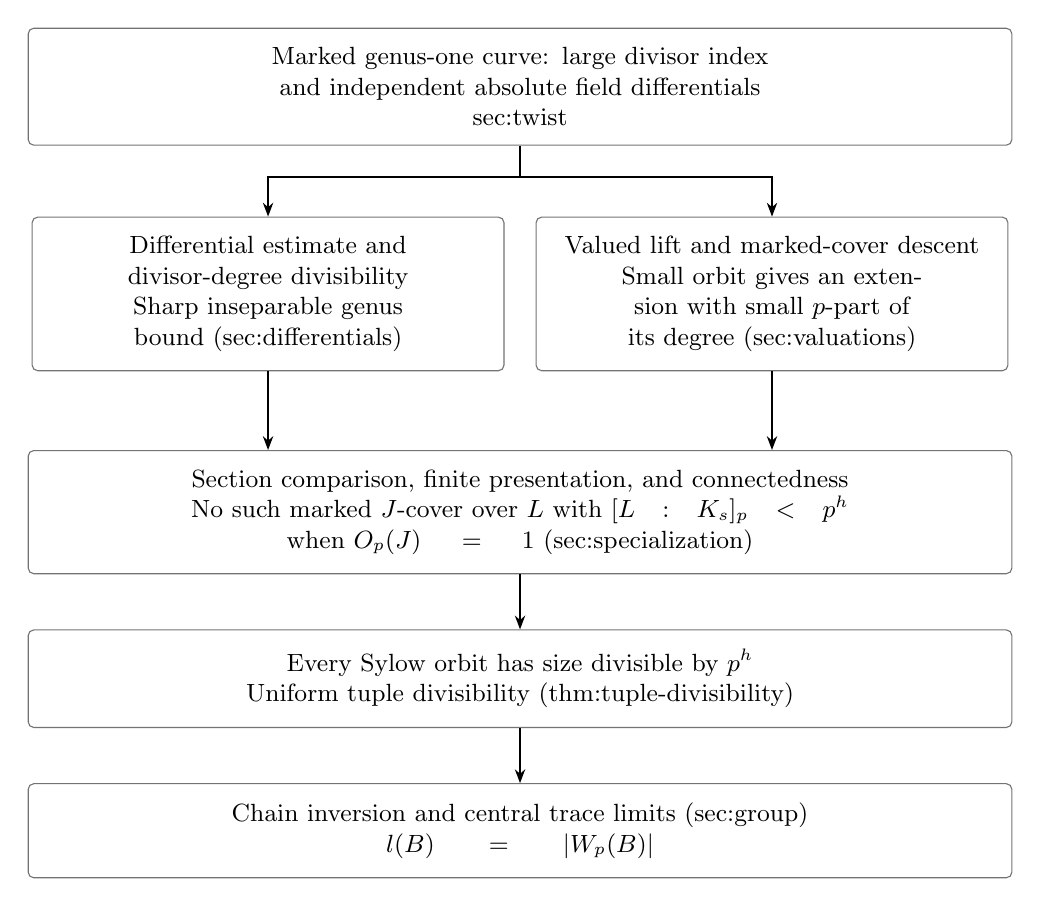
\begin{tikzpicture}[
  every node/.style={font=\small,align=center},
  stage/.style={draw=black!55,rounded corners=2pt,inner sep=7pt},
  flow/.style={-{Stealth[length=5pt]},semithick}
]
\node[stage,text width=12cm] (twist)
  {Marked genus-one curve: large divisor index\\
   and independent absolute field differentials\\
   \Cref{sec:twist}};
\coordinate (branch-top) at ($(twist.south)+(0,-9mm)$);
\coordinate (branch-split) at ($(twist.south)+(0,-4mm)$);
\node[stage,text width=5.5cm,anchor=north] (genus)
  at ($(branch-top)+(-3.2cm,0)$)
  {Differential estimate and divisor-degree divisibility\\Sharp inseparable genus bound
   (\Cref{sec:differentials})};
\node[stage,text width=5.5cm,anchor=north] (lift)
  at ($(branch-top)+(3.2cm,0)$)
  {Valued lift and marked-cover descent\\Small orbit gives an extension
   with small $p$-part of its degree
   (\Cref{sec:valuations})};
\node[fit=(genus)(lift),inner sep=0pt,outer sep=0pt] (branches) {};
\node[stage,text width=12cm,below=10mm of branches] (specialization)
  {Section comparison, finite presentation, and connectedness\\
   No such marked $J$-cover over $L$ with $[L:K_s]_p<p^h$\\
   when $O_p(J)=1$
   (\Cref{sec:specialization})};
\node[stage,text width=12cm,below=7mm of specialization] (count)
  {Every Sylow orbit has size divisible by $p^h$\\
   Uniform tuple divisibility (\Cref{thm:tuple-divisibility})};
\node[stage,text width=12cm,below=7mm of count] (blocks)
  {Chain inversion and central trace limits (\Cref{sec:group})\\
   $l(B)=|W_p(B)|$};
\draw[flow] (twist.south) -- (branch-split) -| (genus.north);
\draw[flow] (twist.south) -- (branch-split) -| (lift.north);
\draw[flow] (genus.south) -- (genus.south |- specialization.north);
\draw[flow] (lift.south) -- (lift.south |- specialization.north);
\draw[flow] (specialization.south) -- (count.north);
\draw[flow] (count.south) -- (blocks.north);
\end{tikzpicture}
\end{document}
